\documentclass[12pt]{article}
\usepackage[english]{babel}
\usepackage[utf8x]{inputenc}
\usepackage{amsmath}
\usepackage{graphicx}
\usepackage{caption}
\usepackage{subcaption}
\usepackage{etoolbox}
\usepackage{changepage}
\usepackage{titlesec}
\usepackage[parfill]{parskip}
\usepackage[margin=1in]{geometry}
\usepackage{times}
\usepackage[numbers,super]{natbib}
\usepackage{float}
\usepackage[T1]{fontenc}

\titleformat*{\section}{\normalsize\bfseries} % Makes section titles 12 pt font


%----------------------------------------------------------------------------------------
%  TITLE SECTION
%----------------------------------------------------------------------------------------
\title{\large \textbf{Twitter in the Engineering Classroom}} % using \large makes the title approximately 14 pt.
\author{\vspace{-5ex}}
\author{\normalsize Devin R. Berg\\
\normalsize bergdev@uwstout.edu\\
\normalsize Engineering and Technology Department\\\
\normalsize University of Wisconsin-Stout}
\date{\vspace{-5ex}} % This leaves the date blank.

\makeatletter % This gets the margins for the title set.
\patchcmd{\@maketitle}{\begin{center}}{\begin{adjustwidth}{0.5in}{0.5in}\begin{center}}{}{}
\patchcmd{\@maketitle}{\end{center}}{\end{center}\end{adjustwidth}}{}{}
\makeatother

\floatstyle{boxed}
\newfloat{textbox}{htbp}{lop}
\floatname{textbox}{Textbox}

%----------------------------------------------------------------------------------------

\begin{document}
\raggedright
\maketitle
\thispagestyle{empty}
\pagestyle{empty}

%----------------------------------------------------------------------------------------
%  PAPER CONTENTS
%----------------------------------------------------------------------------------------
\section*{Abstract}
The micro-blogging platform, Twitter, has been employed by some in higher education as a tool for enhanced student engagement. This platform has shown promise as an educational tool for the promotion of critical reading and writing and concise expression of ideas. However, it is unclear in what settings and under what circumstances Twitter can be effectively employed in the engineering classroom. These questions were explored over a multi-semester study of student participation in directed social media discussions within the engineering classroom. The various cohorts of students included in this study were drawn from engineering courses. Comparisons will be made between these multiple cohorts on the basis of active engagement in the assigned tasks, course performance, concept inventory performance, and student perception of the tasks. Through the process of using this practice in the classroom, it was found that there was difficulty encouraging engineering students to participate in Twitter discussions regardless of the incentive provided. Limited evidence was found of greater course achievement correlating with greater participation in Twitter based tasks. It is expected that greater effort is required in familiarizing students with the Twitter platform and increasing their comfort level with asking questions and carrying out discussions in a public forum.


\section*{Introduction}
The use of social media (SM) in the higher education classroom has expanded in recent years as educators come to realize the benefits of the various SM platforms for use as tools for faculty-student communication or for inter-student communication \cite{blessing_using_2012}. While the literature on the use of SM in the classroom is emerging, recent studies have found the platform functional for promoting concise expression of ideas, critical reading and writing skills, stronger student-teacher relationships, self-learning in an informal environment, and accountability among other benefits \cite{shiffman_twitter_2012}. The use of social media in the classroom might be viewed as a form of inquiry-based learning, an educational approach that allows the student to take ownership over the education process by self-identifying examples relevant to course curriculum, possibly outside of the classroom \cite{magnussen_impact_2000, prince_does_2004}. Benefits of similar educational techniques have been found in relation to asking students to communicate the content of a given course to a broader, general-public audience \cite{junco_effect_2011, ha_influence_2013}. However, at the same time it can be a challenge to promote active participation in this sort of activity due to students’ apprehension engaging in public discourse. Similar apprehensions at the instructor level have limited the use of Twitter as a classroom resource \cite{carpenter_how_2014}. Further, using SM in the classroom has potential disadvantages such as distracting content, overly constraining character limitations, and privacy concerns \cite{dhir_tweeters_2013}. Classes with large enrollments may deter active student engagement as has been noted in the literature \cite{ahlfeldt_measurement_2005}.  

Twitter has been employed by some in higher education as a tool for enhanced student engagement. However, it is unclear in what settings and under what circumstances Twitter can be effectively employed in the engineering classroom. In what ways can we encourage students to develop more effectively through Twitter use in the classroom?


\section*{Methodology}
Twitter was employed as a educational tool across five academic semesters in six course sections with a cumulative total of 195 student participants. An additional 150 students are included for which Twitter was not used to provide a basis for comparison. The distribution of student participants across the various cohorts is shown in Table \ref{cohortDemo}. The application of Twitter in the classroom (treatment) is shown as either being a required component or as ``extra credit'' as appropriate.

\begin{table}[H]
\caption{Cohort demographics including sample size and method by which treatment was applied.}
\begin{center}
\label{cohortDemo}
\begin{tabular}{ccc}
% & & & & &\\ % Some space after the caption.
\hline
 Cohort & Sample Size & Treatment Applied \\
\hline
 A & 26 & none \\ 
 B & 24 & none \\ 
 C & 26 & none \\ 
 D & 20 & none \\ 
 E & 11 & none \\ 
 F & 25 & none \\
 G & 18 & none \\
 H & 16 & required \\ 
 I & 21 & required \\ 
 J & 15 & required \\ 
 K & 46 & required \\ 
 L & 35 & required \\ 
 M & 42 & extra credit \\ 
 N & 20 & extra credit \\ 
\hline
\end{tabular}
\end{center}
\end{table}

The tasks that students were asked to complete as part of the study involved weekly postings to Twitter relevant to the topics of discussion in the course that week. With these tasks, it was intended for the student to look beyond their standard homework and relate to the course material in a new way, independent of their textbook or course notes. Similar work by others has demonstrated success in getting students to make the connection between the classroom and the ``real world'' \cite{hopp_journal_2008}.

The deliverables for these tasks consisted of either discussion, a photograph, or a video that is relevant to the week's course material. The students were also asked to comment on their peer's postings, thus spurring further discussion. Evaluation of student learning outcomes will be discussed and comparisons will be made between the small cohort and large cohort groups.

Twitter was utilized as a means to both collect and promote discussions around student submissions. When posting to Twitter, students were asked to include a course hashtag with each of their posts (tweets) to provide a means of quickly sorting and organizing relevant posts. Students were asked to produce one original submission on an approximately per week schedule corresponding with the submission deadlines for their normal homework assignments. Each original submission was expected to include a photograph or video and a brief descriptive statement that demonstrated  the concepts discussed in that week's lectures. Students were also asked to submit at least two comments on the posts of their classmates. The instructor used limited direct participation in the ongoing Twitter discussion during the first few weeks of the semester in an attempt to spur student participation. After those initial weeks, the instructor posted more sparingly as needed. The majority of instructor participation was centered around course announcements or responses to student questions.

To facilitate archiving of student Twitter posts related to the class, all posts containing the course hashtag were collected and analyzed using the Twitter Archiving Google Spreadsheet (TAGS) \cite{hawksey_twitter_2014}. This tool allowed for automated collection of all tweets tagged appropriately along with the corresponding time stamp and performed high level analysis of the connections (mentions) between tweets.

\section*{Results and Assessment}
The total number of tweets collected in the archive in a given semester varied from 25 for a smaller cohort for which participation was for extra credit only to 931 for a larger cohort with mandatory participation. However, it is important to note that reliable collection of all course tweets was hampered by the limits of the search functionality, as previously mentioned. A comparison of the number of posts for each cohort is shown in Table \ref{participation}.

\begin{table}[H]
\caption{Participation metrics from cohorts for which treatment was applied.}
\begin{center}
\label{participation}
\begin{tabular}{ccc}
% & & & & &\\ % Some space after the caption.
\hline
 Cohort & \# Tweets & Tweets/student \\
\hline
 H & 178 & 11.1 \\
 I & 217 & 10.3 \\
 J & 216 & 14.4 \\
 K & 931 & 20.2 \\
 L & 467 & 13.3 \\
 M & 30 & 0.7 \\
 N & 29 & 1.5 \\
\hline
\end{tabular}
\end{center}
\end{table}

Consistent with what was previously reported, student posts via Twitter were typically \textit{simple} in nature due to the limitations of the platform \cite{berg_evaluation_2014}. Posts primarily consisted of links to existing online content, photos of items relevant to the course content \cite{berg_relationship_2015}, or original videos demonstrating course topics \cite{cleveland_impact_2014}. Comparing student submissions across cohorts suggests that quality and detail of the posts is relatively independent of cohort size \cite{_twitter_}.

Quantitative data was collected across the cohorts. The cohorts were grouped on the basis of treatment type. Cohorts \textit{A-G} had no Twitter use, cohorts \textit{H-L} had required Twitter usage, and cohorts \textit{M} and \textit{N} were only given extra credit for Twitter usage. Along these groupings, the cohorts are compared on the basis of exam scores, cumulative homework score, and final course grade as shown in Table \ref{quantPerformance}. Data is presented as average grouping performance for each group along with standard deviation for each average score. The results show that...

\begin{table}[H]
\caption{Quantitative performance assessment for both cohorts.}
\begin{center}
\label{quantPerformance}
\begin{tabular}{lcccccc}
% & & & & &\\ % Some space after the caption.
\hline
 Twitter Usage & HW & Exam 1 & Exam 2 & Exam 3 & Final Grade\\
\hline
 None & 71.0 $\pm$ 22.3 & 76.8 $\pm$ 16.0 & 67.4 $\pm$ 18.9 & 60.5 $\pm$ 16.7 & 71.6 $\pm$ 14.4\\ 
 Extra Credit & 84.5 $\pm$ 18.2 & 73.5 $\pm$ 13.1 & 74.6 $\pm$ 11.3 & 63.4 $\pm$ 13.9 & 76.6 $\pm$ 6.3\\ 
 Required & 77.6 $\pm$ 19.9 & 80.4 $\pm$ 12.0 & 75.2 $\pm$ 12.9 & 65.3 $\pm$ 14.5 & 76.9 $\pm$ 8.1\\ 
\hline
\end{tabular}
\end{center}
\end{table}

\begin{table}[H]
\caption{Statistical significance calculated using a one-way ANOVA and Tukey post-hoc test, p-values below 0.05 indicate a statistically significant difference between the two compared treatment conditions.}
\begin{center}
\label{ANOVA}
\begin{tabular}{lcccccc}
% & & & & &\\ % Some space after the caption.
\hline
 Treatments Compared & HW & Exam 1 & Exam 2 & Exam 3 & Final Grade\\
\hline
 None | EC & \textless 0.001 & 0.255 & 0.006 & 0.543 & 0.035\\ 
 None | Required & 0.043 & 0.086 & \textless 0.001 & 0.046 & 0.001\\ 
 EC | Required & 0.171 & 0.004 & 0.971 & 0.770 & 0.986\\ 
\hline
\end{tabular}
\end{center}
\end{table}

The grades each student on the cumulative homework, exams, and final course grade versus number of tweets posted is shown in Fig. \ref{fig:numTweets}.

\begin{figure}[hbtp]
\centering
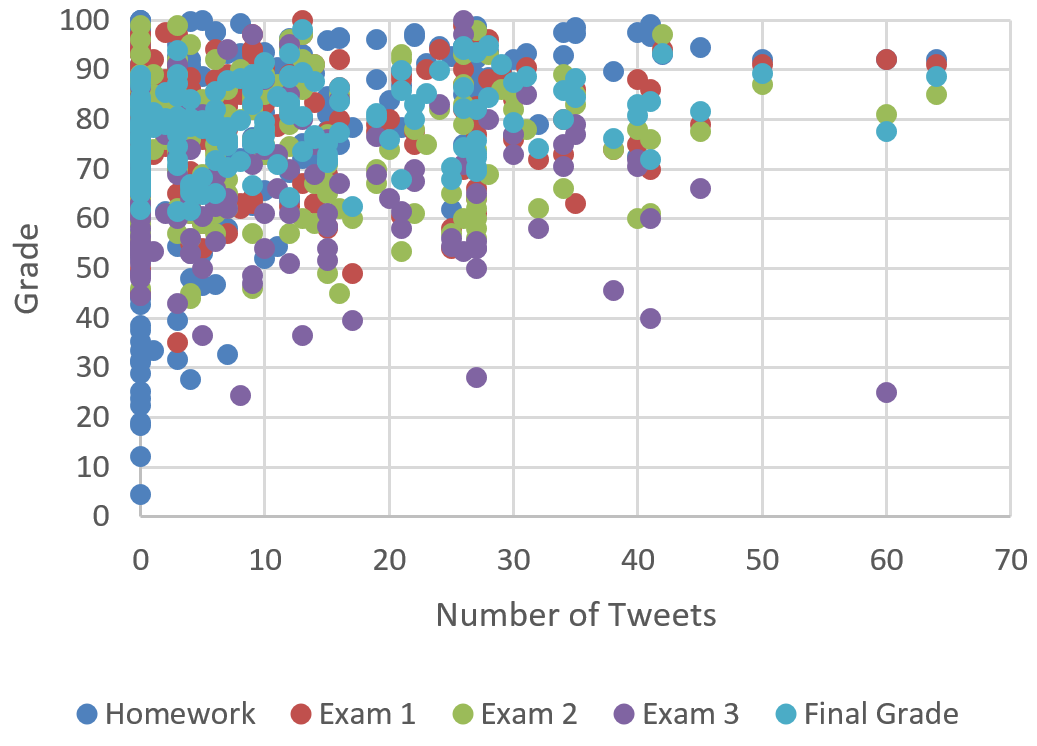
\includegraphics[width=\textwidth]{figures/numTweets.png}
\caption{Homework, exams, and course grades versus number of tweets posted.}
\label{fig:numTweets}
\end{figure}


%------------------------------------------------

\section*{Discussion}
The hypothesis of this study was that a larger cohort of students would lead to greater class participation by cultivating a feeling of anonymity and by increasing the likelihood of the class having an active participant who would drive class participation. However, this hypothesis proved to be false. While the participation measured as tweets per student per assignment was slightly higher for the large cohort, it was still lower than was measured in previous studies. Student outcomes measured using concept inventories and course examinations found little difference between the cohorts with the exception of greater achievement correlated with higher participation for the large cohort relative to the small cohort. Finally, qualitative efficacy survey results showed that the small cohort had slightly better self-reported efficacy compared with the large cohort. In terms of achieving greater student engagement in such an activity, it has been the experience of the author that greater activity is driven largely by have a small number of students who push class participation. However, it would seem that this is not achieved just by virtue of a large class size and does not overcome the limitations of lower student engagement in larger classes as previously observed \cite{ahlfeldt_measurement_2005}. Therefore, some other incentive must be found to promote active participation.

Informally, students have communicated that they had difficulty remembering to complete the required Twitter postings and could often not think of anything to post. Further consideration is needed to determine how to address these issues. The author plans to continue use of this type of activity while finding ways to promote greater participation. For example, opening the assignment to a greater variety of social media platforms such as Facebook or similar may lower the barrier to entry for the students. Additionally, making use of a teaching assistant or past student to model active participation may encourage more students in the course to follow their example. These techniques remain to be explored through further study.


\section*{Acknowledgements}
The author would like to thank the engineering students at the University of Wisconsin-Stout for their photographic and textual contributions.


%----------------------------------------------------------------------------------------
%  REFERENCE LIST
%----------------------------------------------------------------------------------------
\vspace{4\baselineskip}\vspace{-\parskip} % Creaters proper 4 blank line spacing.
\footnotesize % Makes bibliography 10 pt font.
\bibliographystyle{unsrtnat} %Can use a different style as long as it is one which uses numbered references in the text.
\bibliography{refs}

%----------------------------------------------------------------------------------------



\end{document}
